\section{Motivación}

\begin{frame}
	\frametitle{\secname}
	\begin{columns}
		\begin{column}{.38\paperwidth}
			\begin{alertblock}{¿Por qué el método de volúmenes finitos?}
				\begin{enumerate}
					\item

					      Ideal para EDPs escritas en su forma conservativa.
					      \begin{equation}\label{eq:conservationlaw}
						      \difcp{u}{t}+
						      \difcp{f\left(u\right)}{x}=0.
					      \end{equation}

					      \

					\item

					      La discretización a partir de la forma integral.

					      \

					\item

					      No existen esquemas numéricos de diferencias finitas
					      de orden mayor o igual que 2 estables, esto es conocido
					      como el Teorema de Barrera de Godunov.

					      \

					\item

					      Para una ley de conservación hiperbólica, el método de Galerkin
					      conforme no es adecuado, se prefieren variantes como
					      Galerkin-Discontinuo o método estabilizados como
					      Streamline Upwind Petrov-Galerkin.
				\end{enumerate}
			\end{alertblock}
		\end{column}
		\begin{column}{.58\paperwidth}
			\begin{figure}[ht!]
				\centering
				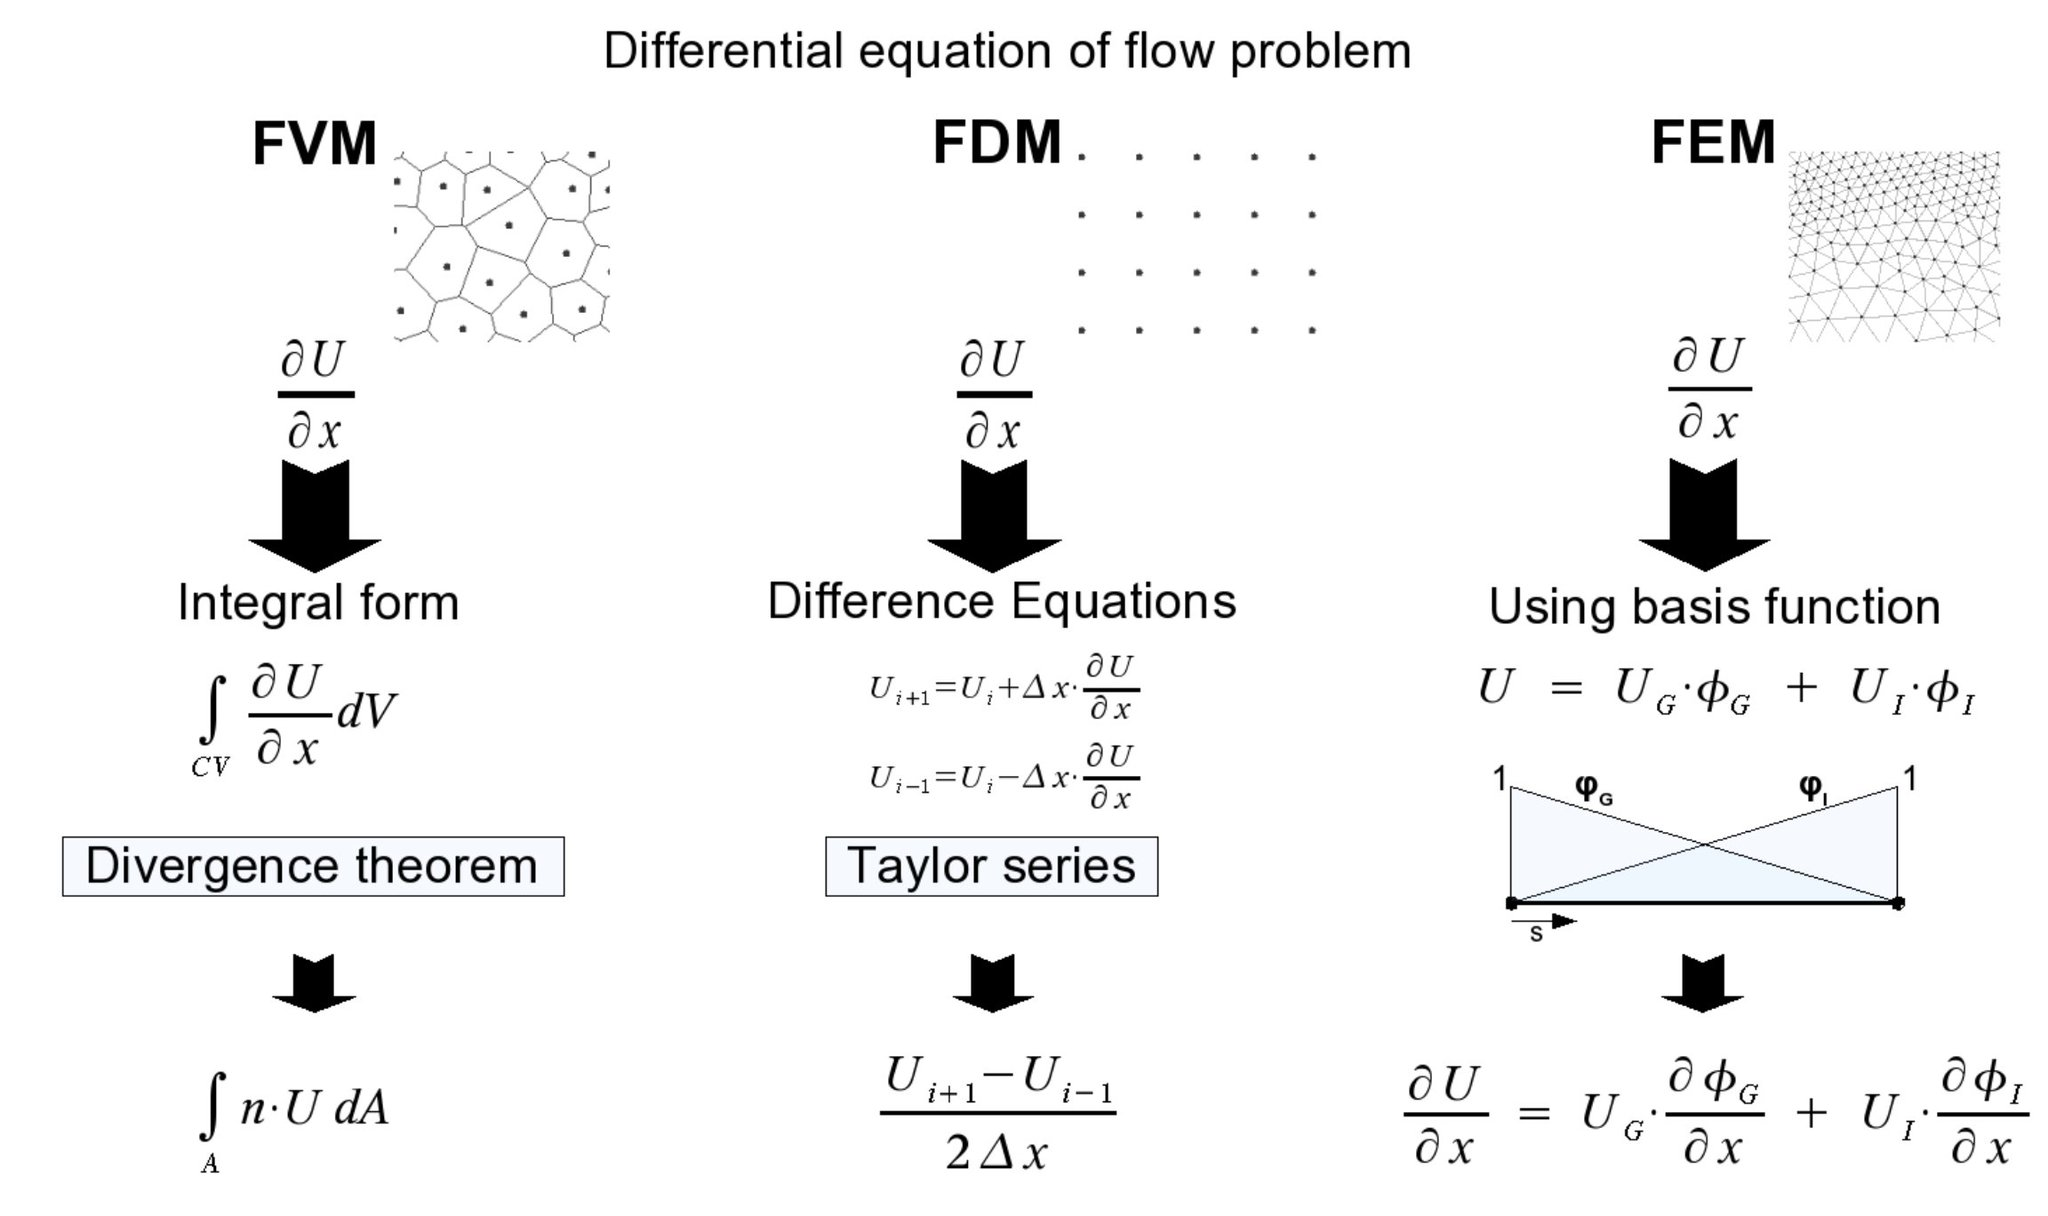
\includegraphics[width=.5\paperwidth]{methods.pdf}
			\end{figure}
		\end{column}
	\end{columns}
\end{frame}
